\subsection{简单线性回归}\label{sec:11.3}\index{SI0878@回归}
在方差分析中，考察了一个因子（变量）怎样影响响应变量的均值. 现在转向简单线性回归，试图更好地理解一个变量对另一个变量的函数依赖. 特别地，在简单线性回归中，有如下形式的关系：
\begin{equation}\label{eq:11.3.1}
Y_i=\alpha+\beta x_i+\varepsilon_i,
\end{equation}
其中$Y_i$为随机变量，$x_i$为另一个可观测变量. $\alpha$与$\beta$分别为回归的截距（intercept）和斜率（slope），假设为固定的未知参数，而$\varepsilon_i$必然是随机变量. 通常还假设$E\varepsilon_i=0$（否则只需将多出的均值调整到$\alpha$中），因此由\eqref{eq:11.3.1}有
\begin{equation}\label{eq:11.3.2}\index{SI0901@总体}
EY_i=\alpha+\beta x_i.
\end{equation}
一般而言，把$EY$表示为$x$的函数的函数称为总体回归函数. \eqref{eq:11.3.2}定义了简单线性回归的总体回归函数.

回归的一个主要目的是利用\eqref{eq:11.3.2}这样的关系，根据已知的$x_i$预测$Y_i$. 日常用语中常将其解释为$Y_i$依赖于$x_i$，并常把$Y_i$称为因变量（dependent variable），$x_i$称为自变量（independent variable）.\index{SI0889@因变量}\semanticindexanchor{889:466}\index{SI0892@自变量}\semanticindexanchor{892:466}
\sourcepageanchor{467}
但这一术语容易引起混淆，因为这里“independent”的含义不同于此前的用法. （$x_i$未必是随机变量，所以不能按通常意义称其为统计上“独立”.）我们不使用这种容易混淆的术语，而采用描述性更强的另一组术语，将$Y_i$称为响应变量（response variable），$x_i$称为预测变量（predictor variable）.\index{SI0903@预测变量}\semanticindexanchor{903:467}\index{SI0906@响应变量}\semanticindexanchor{906:467}

实际上，为明确关于$Y_i$与$x_i$关系的推断以已知$x_i$为前提，可以把\eqref{eq:11.3.2}写为
\begin{equation}\label{eq:11.3.3}\index{SI0884@条件期望}
E(Y_i\mid x_i)=\alpha+\beta x_i.
\end{equation}
我们倾向于使用\eqref{eq:11.3.3}，以强调推断的条件性质.

回顾\autoref{sec:4}，在讨论条件期望时遇到过“回归”一词（见\autoref{exercise:4.13}）. 那里把$Y$对$X$的回归定义为$E(Y\mid x)$，即给定$X=x$时$Y$的条件期望. 更一般地，统计学中“回归”表示变量之间的一种关系. 说回归是线性的，可以指给定$X=x$时$Y$的条件期望是$x$的线性函数. 注意，在\eqref{eq:11.3.3}中，$x_i$是固定已知的，还是可观测随机变量$X_i$的一次实现，并无区别；两种情况下\eqref{eq:11.3.3}的解释相同. 但在\autoref{sec:11.3.4}中将利用$X_i,Y_i$的联合分布进行推断，那时情况就不同了.

术语线性回归是指模型设定\emph{对参数线性}.\index{SI0895@线性}\semanticindexanchor{895:467}\index{SI0896@关于x线性}\semanticindexanchor{896:467} 因而，$E(Y_i\mid x_i)=\alpha+\beta x_i^2$和$E(\log Y_i\mid x_i)=\alpha+\beta(1/x_i)$都规定了线性回归. 前者规定$Y_i$与$x_i^2$之间的线性关系，后者规定$\log Y_i$与$1/x_i$之间的线性关系. 相反，$E(Y_i\mid x_i)=\alpha+\beta^2x_i$并不规定线性回归.

“回归”一词有一段有趣的历史，可追溯至19世纪Francis Galton爵士的工作. （更多细节见\hyperref[bib:source129]{Freedman等（1991）}，深入的历史论述见\hyperref[bib:source308]{Stigler（1986）}.）Galton研究了父亲身高与儿子身高的关系. 不出所料，他发现高个父亲倾向于有高个儿子，矮个父亲倾向于有矮个儿子. 但他也发现，特别高的父亲倾向于有较矮的儿子，特别矮的父亲倾向于有较高的儿子. （想一想——这是有道理的.）Galton把这种现象称为向均值回归（regression toward the mean），\index{SI0910@向均值回归}\semanticindexanchor{910:467}采用“regression”的通常含义“回去”；今天“回归”一词的用法便源于此.

\begin{example}[预测葡萄产量]\label{ex:11.3.1}
回归的一项较现代应用是预测葡萄收成. 七月，葡萄藤结出果串，果串数量可用于预测采收时的最终产量. 典型数据如下，列出若干年的果串数和产量（吨/英亩）.
\begin{center}
\begin{tabular}{rrr}
\toprule 年份&产量（$Y$）&果串数（$x$）\\\midrule
1971&5.6&116.37\\1973&3.2&82.77\\1974&4.5&110.68\\1975&4.2&97.50\\
1976&5.2&115.88\\1977&2.7&80.19\\1978&4.8&125.24\\1979&4.9&116.15\\
1980&4.7&117.36\\1981&4.1&93.31\\1982&4.4&107.46\\1983&5.4&122.30\\\bottomrule
\end{tabular}
\end{center}
1972年的数据缺失，因为那年的作物被飓风摧毁. 这些数据的图形会显示出很强的线性关系.
\end{example}

\sourcepageanchor{468}
写下\eqref{eq:11.3.3}这样的方程时，隐含地假设$Y$对$X$的回归是线性的，即给定$X=x$时$Y$的条件期望是$x$的线性函数. 这一假设未必有依据，因为可能没有支持线性关系的基础理论. 但线性关系处理起来非常方便，所以可能愿意假设$Y$对$X$的回归能用线性函数充分近似. 因而，实际上并不指望\eqref{eq:11.3.3}严格成立，而是希望
\begin{equation}\label{eq:11.3.4}
E(Y_i\mid x_i)\approx\alpha+\beta x_i
\end{equation}
是一种合理的近似. 若从一个（相当强的）假设出发，即$(X_i,Y_i)$服从二元正态分布，就立即得到$Y$对$X$的回归是线性的. 此时条件期望$E(Y\mid x)$对参数线性（见\autoref{def:4.5.10}及其后的讨论）.

最后还需作一个区分. 回归分析，即考察预测变量与响应变量之间的关系，包含两个步骤. 第一步完全以数据为对象，只试图概括观测到的数据.\index{SI0888@数据拟合}\semanticindexanchor{888:468} （这一步总会进行，因为几乎总要计算样本均值、方差或其他汇总统计量；但现在这部分分析往往变得更复杂.）必须记住，这一步“数据拟合”不属于统计推断. 因为只关心手中的数据，不必对参数作任何假设.

回归分析的第二步是统计步骤，试图对总体中的关系，也就是总体回归函数，作推断.\index{SI0893@推断}\semanticindexanchor{893:468} 为此必须对总体作假设. 特别是，若希望对总体线性关系的斜率和截距作推断，就必须假设存在与这些量对应的参数.

简单线性回归问题中，观测数据由$n$对观测$(x_1,y_1),\allowbreak\ldots,\allowbreak(x_n,y_n)$组成. 本节将考虑这些数据的若干不同模型. 各模型对$x$、$y$或二者是否为随机变量$X$、$Y$的观测值有不同假设.

每种模型都关注$x$与$y$之间的线性关系. $n$个数据点不会恰好落在一条直线上，但我们希望通过对观测点拟合直线来概括样本信息. 将看到，许多不同的方法都导向同一条直线.

基于数据$(x_1,y_1),\allowbreak\ldots,\allowbreak(x_n,y_n)$，定义以下各量. 样本均值为
\begin{equation}\label{eq:11.3.5}
\bar x=\frac1n\sum_{i=1}^nx_i\quad\text{且}\quad\bar y=\frac1n\sum_{i=1}^ny_i.
\end{equation}
平方和为
\begin{equation}\label{eq:11.3.6}\index{SI0907@平方和}
S_{xx}=\sum_{i=1}^n(x_i-\bar x)^2\quad\text{且}\quad S_{yy}=\sum_{i=1}^n(y_i-\bar y)^2,
\end{equation}
交叉乘积和为
\begin{equation}\label{eq:11.3.7}
S_{xy}=\sum_{i=1}^n(x_i-\bar x)(y_i-\bar y).
\end{equation}
\eqref{eq:11.3.4}中$\alpha,\beta$最常用的估计分别记为$a,b$，如下给出；稍后将在不同模型下论证它们：
\begin{equation}\label{eq:11.3.8}
b=\frac{S_{xy}}{S_{xx}}\quad\text{且}\quad a=\bar y-b\bar x.
\end{equation}

\sourcepageanchor{469}
\begin{figure}[htbp]
\centering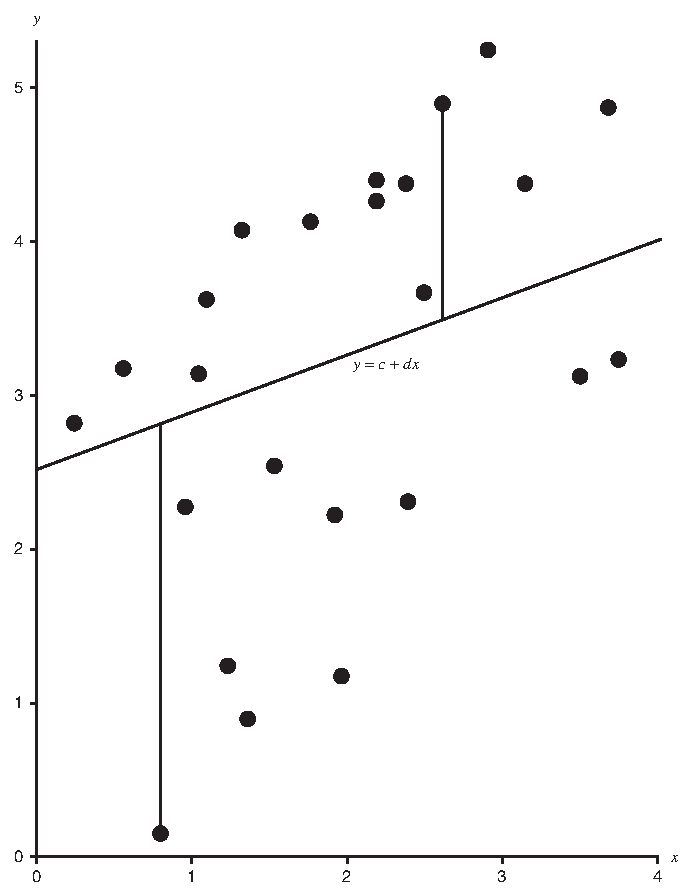
\includegraphics[width=.77\textwidth]{assets/chapter11/fig-11.3.1.pdf}
\caption{\autoref{tab:11.3.1}的数据：RSS所度量的竖直距离}\label{fig:11.3.1}
\end{figure}

\subsubsection{最小二乘：一种数学解法}\label{sec:11.3.1}\index{SI0606@最小二乘估计}
第一次推导$\alpha,\beta$的估计时，不对观测$(x_i,y_i)$作任何统计假设. 只把$(x_1,y_1),\allowbreak\ldots,\allowbreak(x_n,y_n)$看成绘制于散点图中的$n$对数，如\autoref{fig:11.3.1}. （图中24个数据点列于\autoref{tab:11.3.1}.）想象穿过这团点画一条直线，使它“尽可能接近”所有点.

对任意直线$y=c+dx$，定义残差平方和（residual sum of squares，RSS）为\index{SI1013@残差}\semanticindexanchor{1013:469}
$$\mathrm{RSS}=\sum_{i=1}^n\bigl(y_i-(c+dx_i)\bigr)^2.$$
RSS度量每个数据点到直线$c+dx$的\emph{竖直}距离，再将这些距离的平方相加. （\autoref{fig:11.3.1}画出了其中两个距离.）

\sourcepageanchor{470}
\begin{table}[htbp]
\centering\caption{\autoref{fig:11.3.1}中的数据}\label{tab:11.3.1}
\begin{tabular}{*{8}{>{\centering\arraybackslash}p{\dimexpr(\textwidth-16\tabcolsep)/8\relax}}}
\toprule $x$&$y$&$x$&$y$&$x$&$y$&$x$&$y$\\\midrule
3.74&3.22&0.20&2.81&1.22&1.23&1.76&4.12\\
3.66&4.87&2.50&3.71&1.00&3.13&0.51&3.16\\
0.78&0.12&3.50&3.11&1.29&4.05&2.17&4.40\\
2.40&2.31&1.35&0.90&0.95&2.28&1.99&1.18\\
2.18&4.25&2.36&4.39&1.05&3.60&1.53&2.54\\
1.93&2.24&3.13&4.36&2.92&5.39&2.60&4.89\\\midrule
\multicolumn{8}{c}{$\bar x=1.95\quad\bar y=3.18\quad S_{xx}=22.82\quad S_{yy}=43.62\quad S_{xy}=15.48$}\\\bottomrule
\end{tabular}
\end{table}
$\alpha,\beta$的最小二乘估计（least squares estimates）定义为使直线$a+bx$的RSS最小的$a,b$值. 即最小二乘估计$a,b$满足
$$\min_{c,d}\sum_{i=1}^n\bigl(y_i-(c+dx_i)\bigr)^2
=\sum_{i=1}^n\bigl(y_i-(a+bx_i)\bigr)^2.$$

这个关于$c,d$两个变量的函数可如下最小化. 对任意固定的$d$，写成
$$\sum_{i=1}^n\bigl(y_i-(c+dx_i)\bigr)^2=\sum_{i=1}^n\bigl((y_i-dx_i)-c\bigr)^2,$$
便可求出给出最小值的$c$. 由\autoref{thm:5.2.4}，使其最小的$c$值为
\begin{equation}\label{eq:11.3.9}\index{SI0614@截距的}
c=\frac1n\sum_{i=1}^n(y_i-dx_i)=\bar y-d\bar x.
\end{equation}
因此，给定$d$时，RSS的最小值为
\begin{align*}
\sum_{i=1}^n\bigl((y_i-dx_i)-(\bar y-d\bar x)\bigr)^2
&=\sum_{i=1}^n\bigl((y_i-\bar y)-d(x_i-\bar x)\bigr)^2\\
&=S_{yy}-2dS_{xy}+d^2S_{xx}.
\end{align*}
将这个关于$d$的二次函数求导并令导数为零，即得使RSS整体最小的$d$：
\begin{equation}\label{eq:11.3.10}\index{SI0615@斜率的}
d=\frac{S_{xy}}{S_{xx}}.
\end{equation}
由于$d^2$的系数为正，该值确实给出最小值. 因此，由\eqref{eq:11.3.9}和\eqref{eq:11.3.10}，\eqref{eq:11.3.8}的$a,b$就是使残差平方和最小的$c,d$值.

RSS只是度量直线$c+dx$到数据点距离的许多合理方法之一. 例如，也可使用水平距离来代替竖直距离. 这等价于将$y$变量画在横轴、$x$变量画在纵轴，然后像上面那样使用竖直距离. 利用上述结果，交换$x,y$的角色，得到最小二乘直线$\hat x=a'+b'y$，其中
$$b'=\frac{S_{xy}}{S_{yy}}\quad\text{且}\quad a'=\bar x-b'\bar y.$$
把直线重新表达为$y$是$x$的函数，得$\hat y=-(a'/b')+(1/b')x$.

通常，由水平距离得到的直线不同于由竖直距离得到的直线. 利用\autoref{tab:11.3.1}的数值，$y$对$x$的回归（竖直距离）
\sourcepageanchor{471}
为$\hat y=1.86+.68x$. $x$对$y$的回归（水平距离）为$\hat y=-2.31+2.82x$. \autoref{fig:12.2.1}画出这两条直线，以及\autoref{sec:12.2}讨论的第三条直线. 若两条直线相同，则斜率相同，$b/(1/b')$应等于1. 但实际上$b/(1/b')\le1$，只在特殊情况下取等. 注意
$$\frac{b}{1/b'}=bb'=\frac{(S_{xy})^2}{S_{xx}S_{yy}}.$$
在\eqref{eq:4.7.9}的H\"older不等式中取$p=q=2$、$a_i=x_i-\bar x$、$b_i=y_i-\bar y$，得$(S_{xy})^2\le S_{xx}S_{yy}$，所以该比值小于1.\index{SI0568@Hölder}\semanticindexanchor{568:471}

若$x$是预测变量，$y$是响应变量，且考虑由$x$预测$y$，则RSS所度量的竖直距离是合理的，它度量$y_i$与其预测值$\hat y_i=c+dx_i$之间的距离. 但若不对$x,y$作这种区分，另一个合理准则——水平距离——却给出不同的直线，就令人不安.

最小二乘法应当仅被视为对一组数据“拟合直线”的方法，\index{SI0888@数据拟合}\semanticindexanchor{888:471}而不应被视为统计推断方法. 在本节没有对数据使用任何统计模型，因此没有构造置信区间或检验假设的依据. 在本节背景下谈论$a,b$，称它们为最小二乘\emph{解}可能比称最小二乘\emph{估计}更合适，因为它们是最小化RSS这一数学问题的解，而不是从统计模型推导出的估计. 不过，正如将看到的，这些最小二乘解在某些统计模型中具有最优性.

\subsubsection{最优线性无偏估计量：一种统计解法}\label{sec:11.3.2}
本节说明，在相当一般的统计模型下，\eqref{eq:11.3.8}的估计$a,b$在线性无偏估计类中最优. 模型如下：假设$x_1,\ldots,x_n$是已知的固定值. （可把它们看作实验人员在实验室实验中选定并设定的值.）$y_1,\ldots,y_n$是互不相关随机变量$Y_1,\ldots,Y_n$的观测值. 假设$x$与$y$之间的线性关系为
\begin{equation}\label{eq:11.3.11}
EY_i=\alpha+\beta x_i,\qquad i=1,\ldots,n,
\end{equation}
并假设
\begin{equation}\label{eq:11.3.12}
\operatorname{Var}Y_i=\sigma^2.
\end{equation}
$\sigma^2$没有下标，因为假设所有$Y_i$都有相同的（未知）方差. 关于$Y_i$前两阶矩的这些假设，就是本小节推导所需的全部假设. 例如，不必指定$Y_1,\ldots,Y_n$的概率分布.

\eqref{eq:11.3.11}和\eqref{eq:11.3.12}的模型也可以这样表述：假设
\begin{equation}\label{eq:11.3.13}
Y_i=\alpha+\beta x_i+\varepsilon_i,\qquad i=1,\ldots,n,
\end{equation}
其中$\varepsilon_1,\ldots,\varepsilon_n$是互不相关的随机变量，满足
\begin{equation}\label{eq:11.3.14}
E\varepsilon_i=0\quad\text{且}\quad\operatorname{Var}\varepsilon_i=\sigma^2.
\end{equation}
$\varepsilon_1,\ldots,\varepsilon_n$称为随机误差（random errors）. 由于$Y_i$只依赖$\varepsilon_i$，且各$\varepsilon_i$互不相关，所以$Y_i$互不相关. 由\eqref{eq:11.3.13}和\eqref{eq:11.3.14}也容易验证\eqref{eq:11.3.11}、\eqref{eq:11.3.12}中$EY_i$和$\operatorname{Var}Y_i$的表达式.

为推导参数$\alpha,\beta$的估计量，将注意力限制在线性估计量类. 若一个估计量具有形式
\begin{equation}\label{eq:11.3.15}\index{SI0792@线性}
\sum_{i=1}^nd_iY_i,
\end{equation}
\sourcepageanchor{472}
其中$d_1,\ldots,d_n$是已知的固定常数，则称为线性估计量（linear estimator）. （\autoref{exercise:7.39}讨论了总体均值的线性估计量.）在线性估计量类中，再限制为无偏估计量，这就限制了$d_1,\ldots,d_n$允许取的值.

无论参数$\alpha,\beta$的真值为何，斜率$\beta$的无偏估计量必须满足
$$E\sum_{i=1}^nd_iY_i=\beta.$$
这意味着
\begin{align*}
\beta&=E\sum_{i=1}^nd_iY_i=\sum_{i=1}^nd_iEY_i=\sum_{i=1}^nd_i(\alpha+\beta x_i)\\
&=\alpha\left(\sum_{i=1}^nd_i\right)+\beta\left(\sum_{i=1}^nd_ix_i\right).
\end{align*}
这一等式对所有$\alpha,\beta$成立，当且仅当
\begin{equation}\label{eq:11.3.16}
\sum_{i=1}^nd_i=0\quad\text{且}\quad\sum_{i=1}^nd_ix_i=1.
\end{equation}
所以，要使该估计量成为$\beta$的无偏估计量，$d_1,\ldots,d_n$必须满足\eqref{eq:11.3.16}.

在\autoref{sec:7}中，如果一个无偏估计量在所有无偏估计量中方差最小，就称其为“最优”. 类似地，若一个线性无偏估计量在线性无偏估计量中方差最小，就称为最优线性无偏估计量（best linear unbiased estimator，BLUE）. 现在说明，定义估计量$b=S_{xY}/S_{xx}$的选择$d_i=(x_i-\bar x)/S_{xx}$是最优的，因为它产生$\beta$的方差最小的线性无偏估计量. （$d_i$必须是已知的固定常数，而$x_i$是已知固定常数，所以这一选择合法.）

关于记号的说明：记号$S_{xY}$强调它是随机变量$Y_1,\ldots,Y_n$的函数，因而是随机变量. $S_{xY}$也依赖非随机的量$x_1,\ldots,x_n$.

由于$Y_1,\ldots,Y_n$互不相关且方差同为$\sigma^2$，任意线性估计量的方差为
$$\operatorname{Var}\sum_{i=1}^nd_iY_i
=\sum_{i=1}^nd_i^2\operatorname{Var}Y_i
=\sum_{i=1}^nd_i^2\sigma^2=\sigma^2\sum_{i=1}^nd_i^2.$$
因此，$\beta$的BLUE由满足\eqref{eq:11.3.16}并使$\sum_{i=1}^nd_i^2$最小的常数$d_1,\ldots,d_n$定义. （$\sigma^2$不影响在线性估计量上的最小化，因为每个线性估计量的方差都以它为乘数.）

现在可用\autoref{lem:11.2.7}求使其最小的$d_1,\ldots,d_n$. 将引理用于这个最小化问题时，作如下对应，其中左端是\hyperref[lem:11.2.7]{引理11.2.1}中的记号，右端是当前记号.\footnote{译注：原文此处再次写引理11.2.1，实际使用的是\autoref{lem:11.2.7}. 保留原显示编号.} 令
$$k=n,\quad v_i=x_i,\quad c_i=1,\quad a_i=d_i,$$
则$\bar v_c=\bar x$. 若$d_i$具有形式
\begin{equation}\label{eq:11.3.17}
d_i=Kc_i(v_i-\bar v_c)=K(x_i-\bar x),\qquad i=1,\ldots,n,
\end{equation}
则由\autoref{lem:11.2.7}，$d_1,\ldots,d_n$在所有满足$\sum d_i=0$的向量中使
\begin{equation}\label{eq:11.3.18}\index{SI0681@二次函数的最大值}
\frac{(\sum_{i=1}^nd_ix_i)^2}{\sum_{i=1}^nd_i^2}
\end{equation}
达到最大.

\sourcepageanchor{473}
此外，由于
$$\{(d_1,\ldots,d_n):\sum d_i=0,\ \sum d_ix_i=1\}
\subset\{(d_1,\ldots,d_n):\sum d_i=0\},$$
如果形如\eqref{eq:11.3.17}的$d_i$还满足\eqref{eq:11.3.16}，它们当然也在所有满足\eqref{eq:11.3.16}的$d_1,\ldots,d_n$中使\eqref{eq:11.3.18}最大. （取最大值的集合变小，最大值不可能增大.）现在利用\eqref{eq:11.3.17}，有
$$\sum_{i=1}^nd_ix_i=\sum_{i=1}^nK(x_i-\bar x)x_i=KS_{xx}.$$
若$K=1/S_{xx}$，就满足\eqref{eq:11.3.16}的第二个约束. 因此，定义
\begin{equation}\label{eq:11.3.19}\index{SI0882@斜率的最优线性无偏估计量}
d_i=\frac{x_i-\bar x}{S_{xx}},\qquad i=1,\ldots,n,
\end{equation}
就满足\eqref{eq:11.3.16}的两个约束，且这一组$d_i$达到最大值. 最后注意，对所有满足\eqref{eq:11.3.16}的$d_1,\ldots,d_n$，
$$\frac{(\sum_{i=1}^nd_ix_i)^2}{\sum_{i=1}^nd_i^2}=\frac1{\sum_{i=1}^nd_i^2}.$$
因此，对满足\eqref{eq:11.3.16}的$d_1,\ldots,d_n$，最大化\eqref{eq:11.3.18}等价于最小化$\sum d_i^2$. 所以可断定，\eqref{eq:11.3.19}定义的$d_i$在所有满足\eqref{eq:11.3.16}的$d_i$中使$\sum d_i^2$最小，而它们定义的线性无偏估计量
$$b=\sum_{i=1}^n\frac{x_i-\bar x}{S_{xx}}y_i=\frac{S_{xy}}{S_{xx}}$$
就是$\beta$的BLUE.

\autoref{fig:11.3.2}给出了构造$\beta$的BLUE的几何描述，其中取$n=3$. 图中是以$d_1,d_2,d_3$为坐标的三维空间. 两个平面分别代表满足\eqref{eq:11.3.16}两个线性约束的向量$(d_1,d_2,d_3)$，两平面的交线代表同时满足两个等式的向量. 对直线上任意点，$\sum_{i=1}^nd_i^2$是该点到原点$\boldsymbol0$距离的平方. 定义BLUE的向量$(d_1,d_2,d_3)$就是直线上距原点最近的点. 图中的球面是与直线相交的最小球面，交点就是定义$\beta$的BLUE的点$(d_1,d_2,d_3)$. 已经证明，该点满足$d_i=(x_i-\bar x)/S_{xx}$.

$b$的方差为
\begin{equation}\label{eq:11.3.20}
\operatorname{Var}b=\sigma^2\sum_{i=1}^nd_i^2=\frac{\sigma^2}{S_{xx}}
=\frac{\sigma^2}{\sum_{i=1}^n(x_i-\bar x)^2}.
\end{equation}
由于$x_1,\ldots,x_n$是实验人员选定的值，\index{SI0890@设计}\semanticindexanchor{890:473}可以选取它们，使$S_{xx}$较大而估计量方差较小. 也就是说，实验人员可通过设计实验使估计更精确. 假设所有$x_1,\ldots,x_n$都必须在区间$[e,f]$中选取. 若$n$为偶数，使$S_{xx}$尽可能大的选择是令一半$x_i$等于$e$，另一半等于$f$（\autoref{exercise:11.26}）. 若实验人员确信\eqref{eq:11.3.11}和\eqref{eq:11.3.12}的模型正确，这就是最优设计，因为它给出斜率$\beta$最精确的估计. 然而实践中很少使用这种设计，因为实验人员几乎从不确信模型. 这种两点设计只提供$x=e$和$x=f$两个值处的$E(Y\mid x)$信息. 如果将$Y$的均值表示为$x$函数的总体回归函数$E(Y\mid x)$是非线性的，从这种“最优”两点设计所得数据中永远无法发现这一点.

\sourcepageanchor{474}
\begin{figure}[htbp]
\centering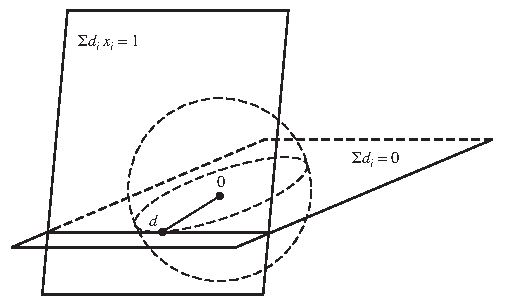
\includegraphics[width=.65\textwidth]{assets/chapter11/fig-11.3.2.pdf}
\caption{BLUE的几何描述}\label{fig:11.3.2}
\end{figure}
已经证明$b$是$\beta$的BLUE. 类似分析可说明$a$是截距$\alpha$的BLUE. 定义$\alpha$的线性估计量的常数$d_1,\ldots,d_n$必须满足
\begin{equation}\label{eq:11.3.21}\index{SI0881@截距的最优线性无偏估计量}
\sum_{i=1}^nd_i=1\quad\text{且}\quad\sum_{i=1}^nd_ix_i=0.
\end{equation}
推导细节留作\autoref{exercise:11.27}. 最小二乘估计量为BLUE这一事实也在其他线性模型中成立.\index{SI0451@Gauss–Markov定理}\semanticindexanchor{451:474} 这个一般结果称为Gauss--Markov定理（Gauss--Markov Theorem）（见\hyperref[bib:source75]{Christensen，1996}；\hyperref[bib:source200]{Lehmann和Casella，1998}，第3.4节；更一般的论述见\hyperref[bib:source160]{Harville，1981）}.

\subsubsection{模型与分布假设}\label{sec:11.3.3}\index{SI0895@线性}
本节再为配对数据$(x_1,y_1),\allowbreak\ldots,\allowbreak(x_n,y_n)$引入两个模型，称为简单线性回归模型.

为了得到\hyperref[sec:11.3.1]{第12.2.1节}中的最小二乘估计，我们没有使用统计模型，而只是解了一个数学上的最小化问题. 因为没有概率模型可用，所以不能推导这种方法所得估计量的任何统计性质. 实际上也没有可为之构造假设检验或置信区间的参数.\footnote{译注：原文写第12.2.1节，但这里回顾的是\autoref{sec:11.3.1}的最小二乘推导. 保留原显示节号.}

在\autoref{sec:11.3.2}，对数据作了一些统计假设. 具体而言，对数据前两阶矩——均值、方差和协方差——作了假设. 它们都是与数据概率模型有关的统计假设，据此推导了估计量的统计性质. 对参数$\alpha,\beta$的估计量$a,b$证明的无偏性和最小方差性质，都属于统计性质.

为得到这些性质，无须指定数据的完整概率模型，只需关于前两阶矩的假设. 在这些最低限度的假设下，得到了一种一般最优性，但只限于受限估计量类——线性无偏估计量. 在该模型下无法推导精确检验与置信区间，因为模型对数据概率分布规定得还不够. 下面给出两个完整规定数据概率结构的统计模型.

\paragraph{11.3.3.1\quad 条件正态模型}\label{sec:11.3.3.1}\index{SI0885@条件正态}
条件正态模型（conditional normal model）是最常见、分析起来最直接的简单线性回归模型. 观测数据为$n$对$(x_1,y_1),\allowbreak\ldots,\allowbreak(x_n,y_n)$. 预测变量的值$x_1,\ldots,x_n$视为已知的固定常数. 如\autoref{sec:11.3.2}，可认为它们是实验人员选定并设定的值.
\sourcepageanchor{475}
响应变量的值$y_1,\ldots,y_n$是随机变量$Y_1,\ldots,Y_n$的观测值. 假设$Y_1,\ldots,Y_n$相互独立，并且$Y_i$服从正态分布，具体为
\begin{equation}\label{eq:11.3.22}
Y_i\sim\mathrm n(\alpha+\beta x_i,\sigma^2),\qquad i=1,\ldots,n.
\end{equation}
所以总体回归函数是$x$的线性函数，即$E(Y\mid x)=\alpha+\beta x$，所有$Y_i$的方差同为$\sigma^2$. 条件正态模型可表示成类似\eqref{eq:11.3.13}、\eqref{eq:11.3.14}的形式：
\begin{equation}\label{eq:11.3.23}
Y_i=\alpha+\beta x_i+\varepsilon_i,\qquad i=1,\ldots,n,
\end{equation}
其中$\varepsilon_1,\ldots,\varepsilon_n$独立同分布于$\mathrm n(0,\sigma^2)$.

条件正态模型是\autoref{sec:11.3.2}所考虑模型的特例. 总体回归函数$E(Y\mid x)=\alpha+\beta x$和方差$\operatorname{Var}Y=\sigma^2$都与该模型相同. $Y_1,\ldots,Y_n$（等价地，$\varepsilon_1,\ldots,\varepsilon_n$）的不相关性被加强为独立性. 当然，现在不仅指定$Y_1,\ldots,Y_n$分布的前两阶矩，还指定了概率分布的精确形式.

由于独立性，$Y_1,\ldots,Y_n$的联合pdf为边缘pdf的乘积，即
\begin{equation}\label{eq:11.3.24}
\begin{aligned}
f(\boldsymbol y\mid\alpha,\beta,\sigma^2)
&=f(y_1,\ldots,y_n\mid\alpha,\beta,\sigma^2)\\
&=\prod_{i=1}^nf(y_i\mid\alpha,\beta,\sigma^2)\\
&=\prod_{i=1}^n\frac1{\sqrt{2\pi}\sigma}\exp\left[-\frac{(y_i-(\alpha+\beta x_i))^2}{2\sigma^2}\right]\\
&=\frac1{(2\pi)^{n/2}\sigma^n}\exp\left[-\frac{\sum_{i=1}^n(y_i-\alpha-\beta x_i)^2}{2\sigma^2}\right].
\end{aligned}
\end{equation}
\autoref{sec:11.3.4}和\autoref{sec:11.3.5}将使用这一联合概率分布建立统计程序. 例如，用\eqref{eq:11.3.24}求$\alpha,\beta,\sigma^2$的MLE.

\paragraph{11.3.3.2\quad 二元正态模型}\label{sec:11.3.3.2}\index{SI0880@二元正态}
此前讨论的所有模型中，预测变量的值$x_1,\ldots,x_n$都是固定的已知常数. 但有时这些值实际上是随机变量$X_1,\ldots,X_n$的观测值. 在\autoref{sec:11.3}的Galton例子中，$x_1,\ldots,x_n$是观测到的父亲身高，实验人员显然没有在收集数据前选定这些身高. 因此必须考虑预测变量和响应变量都随机的模型. 一种相当简单的模型是二元正态模型（bivariate normal model）. \autoref{sec:12.2}将讨论更复杂的模型.

在二元正态模型中，数据$(x_1,y_1),\allowbreak\ldots,\allowbreak(x_n,y_n)$是二元随机向量$(X_1,Y_1),\allowbreak\ldots,\allowbreak(X_n,Y_n)$的观测值. 各随机向量独立，且假设$(X_i,Y_i)$的联合分布为二元正态. 具体假设为
$$ (X_i,Y_i)\sim\text{二元正态}(\mu_X,\mu_Y,\sigma_X^2,\sigma_Y^2,\rho). $$
二元正态分布的联合pdf及各种性质，见\autoref{def:4.5.10}及其后的讨论. 全部数据$(X_1,Y_1),\allowbreak\ldots,\allowbreak(X_n,Y_n)$的联合pdf是这些二元pdf的乘积.

在简单线性回归分析中，仍把$x$看成预测变量，$y$看成响应变量，即最关心的是观测$x$值以后预测$y$值.
\sourcepageanchor{476}
这自然引导我们基于给定$X=x$时$Y$的条件分布进行推断. 对二元正态模型，给定$X=x$时$Y$的条件分布为正态. 总体回归函数现在确实是一个条件期望，正如记号所提示的那样，且为
\begin{equation}\label{eq:11.3.25}
E(Y\mid x)=\mu_Y+\rho\frac{\sigma_Y}{\sigma_X}(x-\mu_X)
=\left[\mu_Y-\rho\frac{\sigma_Y}{\sigma_X}\mu_X\right]
+\left[\rho\frac{\sigma_Y}{\sigma_X}\right]x.
\end{equation}
二元正态模型\emph{蕴含}总体回归是$x$的线性函数，无须像此前模型那样另外假设. 这里$E(Y\mid x)=\alpha+\beta x$，其中$\beta=\rho\sigma_Y/\sigma_X$，$\alpha=\mu_Y-\rho(\sigma_Y/\sigma_X)\mu_X$. 与条件正态模型一样，响应变量$Y$的条件方差也不依赖$x$：
\begin{equation}\label{eq:11.3.26}
\operatorname{Var}(Y\mid x)=\sigma_Y^2(1-\rho^2).
\end{equation}

对二元正态模型，线性回归分析几乎总是利用给定$X_1=x_1,\ldots,X_n=x_n$时$(Y_1,\ldots,Y_n)$的条件分布，而非$(X_1,Y_1),\allowbreak\ldots,\allowbreak(X_n,Y_n)$的无条件分布. 这样就回到上面描述的条件正态模型的情形. 只要以$x_1,\ldots,x_n$为条件，它们原本是随机变量观测值这一事实就无关紧要. 一般而言，简单线性回归中除用二元正态性确定条件分布外，并不使用二元正态性. （事实上，在大多数情况下，$X$的边缘分布完全无关紧要；线性回归中重要的是条件分布.）两种模型基于点估计量、区间或检验的推断相同. 另一种观点见\hyperref[bib:source52]{Brown（1990b）}.

\subsubsection{正态误差下的估计与检验}\label{sec:11.3.4}\index{SI0898@最大似然估计量}
本小节及下一小节在条件正态模型，即\eqref{eq:11.3.22}或\eqref{eq:11.3.23}定义的回归模型下建立推断程序.

首先求三个参数$\alpha,\beta,\sigma^2$的最大似然估计. 由\eqref{eq:11.3.24}的联合pdf，对数似然函数为
$$\log L(\alpha,\beta,\sigma^2\mid\boldsymbol x,\boldsymbol y)
=-\frac n2\log(2\pi)-\frac n2\log\sigma^2
-\frac{\sum_{i=1}^n(y_i-\alpha-\beta x_i)^2}{2\sigma^2}.$$
对任意固定的$\sigma^2$，使$\log L$作为$\alpha,\beta$的函数最大的值$\hat\alpha,\hat\beta$，就是使
$$\sum_{i=1}^n(y_i-\alpha-\beta x_i)^2$$
最小的值. 但这个函数就是\autoref{sec:11.3.1}中的RSS！那里已求得使其最小的值为
$$\hat\beta=b=\frac{S_{xy}}{S_{xx}}\quad\text{且}\quad
\hat\alpha=a=\bar y-b\bar x=\bar y-\hat\beta\bar x.$$
所以$\alpha,\beta$的最小二乘估计也是它们的MLE. 对任意固定的$\sigma^2$，$\hat\alpha,\hat\beta$都是使其最大的值. 现在将它们代入对数似然，为求$\sigma^2$的MLE，只需最大化
$$-\frac n2\log(2\pi)-\frac n2\log\sigma^2
-\frac{\sum_{i=1}^n(y_i-\hat\alpha-\hat\beta x_i)^2}{2\sigma^2}.$$
这与通常正态抽样中求$\sigma^2$的MLE类似（\autoref{ex:7.2.11}），细节留作\autoref{exercise:11.28}. 条件正态模型下$\sigma^2$的MLE为
$$\hat\sigma^2=\frac1n\sum_{i=1}^n(y_i-\hat\alpha-\hat\beta x_i)^2,$$
\sourcepageanchor{477}
即在最小二乘直线处计算的RSS除以样本量. 此后提到RSS，均指在最小二乘直线处计算的RSS.

\autoref{sec:11.3.2}说明$\hat\alpha,\hat\beta$是$\alpha,\beta$的线性无偏估计量. 但$\hat\sigma^2$并不是$\sigma^2$的无偏估计量. 计算$E\hat\sigma^2$以及后续许多计算时，下面的引理会有用.

\begin{lemma}\label{lem:11.3.2}
设$Y_1,\ldots,Y_n$是互不相关的随机变量，且对所有$i=1,\ldots,n$有$\operatorname{Var}Y_i=\sigma^2$. 设$c_1,\ldots,c_n$与$d_1,\ldots,d_n$是两组常数，则
$$\operatorname{Cov}\left(\sum_{i=1}^nc_iY_i,\sum_{i=1}^nd_iY_i\right)
=\left(\sum_{i=1}^nc_id_i\right)\sigma^2.$$
\end{lemma}
\begin{proof}
此前已遇到过此类结果，它类似于\autoref{lem:5.3.3}和\autoref{exercise:11.11}. 不过，这里既不需要$Y_1,\ldots,Y_n$正态，也不需要它们独立.
\end{proof}

接下来求$\sigma^2$中的偏倚.\index{SI0899@有偏}\semanticindexanchor{899:477}\footnote{译注：原文此句写“$\sigma^2$中的偏倚”，实际计算的是估计量$\hat\sigma^2$的偏倚.} 由\eqref{eq:11.3.23}有
$$\varepsilon_i=Y_i-\alpha-\beta x_i.$$
定义回归残差（residuals）为
\begin{equation}\label{eq:11.3.27}\index{SI0905@残差}
\hat\varepsilon_i=Y_i-\hat\alpha-\hat\beta x_i,
\end{equation}
因而
$$\hat\sigma^2=\frac1n\sum_{i=1}^n\hat\varepsilon_i^2=\frac1n\mathrm{RSS}.$$
经计算（\autoref{exercise:11.29}）可得
$$E\hat\varepsilon_i=0,$$
再经过较长的计算（同见\autoref{exercise:11.29}），得
\begin{equation}\label{eq:11.3.28}
\operatorname{Var}\hat\varepsilon_i=E\hat\varepsilon_i^2
=\left(\frac{n-2}n+\frac1{S_{xx}}\left(\frac1n\sum_{j=1}^nx_j^2+x_i^2-2(x_i-\bar x)^2-2x_i\bar x\right)\right)\sigma^2.
\end{equation}
因此
\begin{align*}
E\hat\sigma^2
&=\frac1n\sum_{i=1}^nE\hat\varepsilon_i^2\\
&=\frac1n\sum_{i=1}^n\left[\frac{n-2}n+\frac1{S_{xx}}\left(\frac1n\sum_{j=1}^nx_j^2+x_i^2-2(x_i-\bar x)^2-2x_i\bar x\right)\right]\sigma^2\\
&=\left[\frac{n-2}n+\frac1{nS_{xx}}\left\{\sum_{j=1}^nx_j^2+\sum_{i=1}^nx_i^2-2S_{xx}-\frac2n\left(\sum_{i=1}^nx_i\right)^2\right\}\right]\sigma^2\\
&\hspace{7em}\text{（因为 }\sum x_i\bar x=\tfrac1n(\sum x_i)^2\text{）}\\
&=\left(\frac{n-2}n+0\right)\sigma^2
\qquad\text{（因为 }\sum x_i^2-\tfrac1n(\sum x_i)^2=S_{xx}\text{）}\\
&=\frac{n-2}n\sigma^2.
\end{align*}

\sourcepageanchor{478}
MLE $\hat\sigma^2$是$\sigma^2$的有偏估计量. 更常用的$\sigma^2$估计量是无偏的，定义为
\begin{equation}\label{eq:11.3.29}
S^2=\frac n{n-2}\hat\sigma^2
=\frac1{n-2}\sum_{i=1}^n(y_i-\hat\alpha-\hat\beta x_i)^2
=\frac1{n-2}\sum_{i=1}^n\hat\varepsilon_i^2.
\end{equation}
要基于这些估计量建立估计和检验程序，需要知道其抽样分布. 下面的定理将其汇总.

\begin{theorem}\label{thm:11.3.3}\index{SI0900@抽样分布}
在条件正态回归模型\eqref{eq:11.3.22}下，估计量$\hat\alpha,\hat\beta,S^2$的抽样分布为
$$\hat\alpha\sim\mathrm n\left(\alpha,\frac{\sigma^2}{nS_{xx}}\sum_{i=1}^nx_i^2\right),
\qquad\hat\beta\sim\mathrm n\left(\beta,\frac{\sigma^2}{S_{xx}}\right),$$
并有
$$\operatorname{Cov}(\hat\alpha,\hat\beta)\frac{-\sigma^2\bar x}{S_{xx}}.$$
\footnote{译注：原书协方差式中漏排等号；应读作$\operatorname{Cov}(\hat\alpha,\hat\beta)=-\sigma^2\bar x/S_{xx}$. 此处保留原式.}
此外，$(\hat\alpha,\hat\beta)$与$S^2$独立，且
$$\frac{(n-2)S^2}{\sigma^2}\sim\chi^2_{n-2}.$$
\end{theorem}
\begin{proof}
首先说明$\hat\alpha,\hat\beta$具有所述正态分布. 二者都是独立正态随机变量$Y_1,\ldots,Y_n$的线性函数，所以由\autoref{cor:4.6.10}，二者均为正态分布. 具体而言，\autoref{sec:11.3.2}证明了$\hat\beta=\sum_{i=1}^nd_iY_i$，其中$d_i$由\eqref{eq:11.3.19}给出，并证明了
$$E\hat\beta=\beta\quad\text{且}\quad\operatorname{Var}\hat\beta=\frac{\sigma^2}{S_{xx}}.$$
估计量$\hat\alpha=\bar Y-\hat\beta\bar x$可表示为$\hat\alpha=\sum_{i=1}^nc_iY_i$，其中
$$c_i=\frac1n-\frac{(x_i-\bar x)\bar x}{S_{xx}},$$
因此容易验证
$$E\hat\alpha=\sum_{i=1}^nc_iEY_i
=\sum_{i=1}^n\left(\frac1n-\frac{(x_i-\bar x)\bar x}{S_{xx}}\right)(\alpha+\beta x_i)=\alpha,$$
以及
$$\operatorname{Var}\hat\alpha=\sigma^2\sum_{i=1}^nc_i^2
=\sigma^2\left[\frac1{nS_{xx}}\sum_{i=1}^nx_i^2\right],$$
从而$\hat\alpha,\hat\beta$具有指定的分布. 利用\autoref{lem:11.3.2}也容易求出$\operatorname{Cov}(\hat\alpha,\hat\beta)$. 细节留作\autoref{exercise:11.30}.

接下来说明$\hat\alpha,\hat\beta$与$S^2$独立，这将由\autoref{lem:11.3.2}和\autoref{lem:5.3.3}得到. 根据\eqref{eq:11.3.27}对$\hat\varepsilon_i$的定义，可写为\footnote{译注：原式求和指标是$j$，但最后的随机变量写成$Y_i$；由残差定义应为$Y_j$. 原式照录.}
\begin{equation}\label{eq:11.3.30}
\hat\varepsilon_i=\sum_{j=1}^n[\delta_{ij}-(c_j+d_jx_i)]Y_i,
\end{equation}
其中
$$\delta_{ij}=\begin{cases}1,&i=j,\\0,&i\ne j,\end{cases}
\qquad c_j=\frac1n-\frac{(x_j-\bar x)\bar x}{S_{xx}},\qquad d_j=\frac{x_j-\bar x}{S_{xx}}.$$

\sourcepageanchor{479}
由于$\hat\alpha=\sum c_iY_i$、$\hat\beta=\sum d_iY_i$，应用\autoref{lem:11.3.2}再作一些代数运算，可得
$$\operatorname{Cov}(\hat\varepsilon_i,\hat\alpha)=\operatorname{Cov}(\hat\varepsilon_i,\hat\beta)=0,\qquad i=1,\ldots,n.$$
细节留作\autoref{exercise:11.31}. 因此，由\autoref{lem:5.3.3}，在正态抽样下，$S^2=\sum\hat\varepsilon_i^2/(n-2)$与$\hat\alpha,\hat\beta$独立.

为证明$(n-2)S^2/\sigma^2\sim\chi^2_{n-2}$，将$(n-2)S^2$写成$n-2$个相互独立、各服从$\chi^2_1$分布的随机变量之和.\footnote{译注：此句遗漏除以$\sigma^2$的标准化. 下述系数除已列条件外，还应取为与$(x_1,\ldots,x_n)$正交且各列单位长度，使对应线性组合均值为0、方差为$\sigma^2$；原文明确略去细节，所列内容照录.} 即找常数$a_{ij}$，$i=1,\ldots,n$，$j=1,\ldots,n-2$，满足
\begin{equation}\label{eq:11.3.31}
\sum_{i=1}^n\hat\varepsilon_i^2
=\sum_{j=1}^{n-2}\left(\sum_{i=1}^na_{ij}Y_i\right)^2,
\end{equation}
其中
$$\sum_{i=1}^na_{ij}=0,\quad j=1,\ldots,n-2,
\qquad\text{且}\qquad\sum_{i=1}^na_{ij}a_{ij'}=0,\quad j\ne j'.$$
由于$x_i$具有一般性，细节较为繁复，故略去.
\end{proof}

线性回归的RSS包含了高阶多项式拟合相较线性拟合是否有价值的信息. 由于本模型假设总体回归线性，高阶拟合中的变异只是随机变异. \hyperref[bib:source257]{Robson（1959）}给出了寻找这类高阶多项式拟合系数的一般递推公式，经调整可明确求出\eqref{eq:11.3.31}中的$a_{ij}$. 另外，也可以用Cochran定理（\hyperref[sec:11.5.1]{杂录11.5.1}）证明$\sum\hat\varepsilon_i^2/\sigma^2\sim\chi^2_{n-2}$.

关于两个参数$\alpha,\beta$的推断通常基于以下两个Student $t$分布，它们立即由\autoref{thm:11.3.3}中的正态分布、卡方分布及独立性得到：
\begin{equation}\label{eq:11.3.32}
\frac{\hat\alpha-\alpha}{S\sqrt{(\sum_{i=1}^nx_i^2)/(nS_{xx})}}\sim t_{n-2},
\end{equation}
以及
\begin{equation}\label{eq:11.3.33}\index{SI0908@t统计量}
\frac{\hat\beta-\beta}{S/\sqrt{S_{xx}}}\sim t_{n-2}.
\end{equation}
这两个$t$统计量的联合分布称为二元Student $t$分布\index{SI0275@二元t}\semanticindexanchor{275:479}（bivariate Student's $t$ distribution），其推导方式类似单变量情形. 这里利用了$\hat\alpha,\hat\beta$的联合分布为二元正态，以及两个单变量$t$统计量使用同一个方差估计$S$. 若要对$\alpha,\beta$作同时推断，就要使用这个联合分布. 不过，这里只处理一次关于一个参数的推断.

通常人们对$\beta$比对$\alpha$更感兴趣. 参数$\alpha$是$x=0$时$Y$的期望，即$E(Y\mid x=0)$. 依具体问题而定，这可能是有意义的量，也可能不是. 特别地，$x=0$未必是预测变量的合理取值. 但$\beta$是$E(Y\mid x)$作为$x$函数的变化率，即$x$改变一个单位时$E(Y\mid x)$的改变量. 所以这个参数涉及整个$x$值范围，包含$Y$与$x$之间一切线性关系的信息. （见\autoref{exercise:11.33}.）此外，$\beta=0$这一值尤其值得关注.

若$\beta=0$，则$E(Y\mid x)=\alpha+\beta x=\alpha$，且$Y\sim\mathrm n(\alpha,\sigma^2)$，不依赖$x$. 对一个经过周密思考、准备进行回归分析的实验，我们并不预期会如此，但若事实确实如此，也希望知道.

检验$\beta=0$与ANOVA中检验所有处理相等十分相似. ANOVA的原假设表示，处理与响应在任何方面都无关系；线性回归的原假设$\beta=0$则表示，处理（$x$）与响应之间没有线性关系.

\sourcepageanchor{480}
要检验
\begin{equation}\label{eq:11.3.34}
H_0:\quad\beta=0\quad\text{对}\quad H_1:\quad\beta\ne0,
\end{equation}
利用\eqref{eq:11.3.33}，当
$$\left|\frac{\hat\beta-0}{S/\sqrt{S_{xx}}}\right|>t_{n-2,\alpha/2}$$
时在水平$\alpha$拒绝$H_0$；等价地，当
\begin{equation}\label{eq:11.3.35}\index{SI0909@t检验}
\frac{\hat\beta^2}{S^2/S_{xx}}>F_{1,n-2,\alpha}
\end{equation}
时拒绝. 回顾$\hat\beta$的公式以及$\mathrm{RSS}=\sum\hat\varepsilon_i^2$，有
$$\frac{\hat\beta^2}{S^2/S_{xx}}
=\frac{S_{xy}^2/S_{xx}}{\mathrm{RSS}/(n-2)}
=\frac{\text{回归平方和}}{\text{残差平方和}/\text{自由度}}.$$
最后这个公式汇总在回归ANOVA表中，类似\autoref{sec:11.2}中的ANOVA表. 简单线性回归对应的表见\autoref{tab:11.3.2}，产生\eqref{eq:11.3.35}给出的检验. 注意，表中只涉及关于$\beta$的假设. 参数$\alpha$与估计$\hat\alpha$在这里起的作用，与\autoref{sec:11.2}的总均值相同：只是确定数据的总体水平，在平方和中已被“校正”掉.

\begin{table}[htbp]
\centering\caption{简单线性回归的ANOVA表}\label{tab:11.3.2}\index{SI0879@方差分析表}
\small
\begin{tabular}{lcp{.23\textwidth}p{.22\textwidth}c}
\toprule 变异来源&自由度&平方和&均方&$F$统计量\\\midrule
回归（斜率）&1&回归SS=$S_{xy}^2/S_{xx}$&MS(回归)=回归SS&$F=\dfrac{\mathrm{MS}(\text{回归})}{\mathrm{MS}(\text{残差})}$\\[1ex]
残差&$n-2$&$\mathrm{RSS}=\sum\hat\varepsilon_i^2$&MS(残差)=\newline$\mathrm{RSS}/(n-2)$&\\[1ex]
总计&$n-1$&$\mathrm{SST}=\sum(y_i-\bar y)^2$&&\\\bottomrule
\end{tabular}
\end{table}

\begin{example}[\autoref{ex:11.3.1}续]\label{ex:11.3.4}
葡萄产量数据的回归ANOVA如下.
\begin{center}
葡萄数据的ANOVA表

\begin{tabular}{lrrrr}
\toprule 变异来源&自由度&平方和&均方&$F$统计量\\\midrule
回归&1&6.66&6.66&50.23\\
残差&10&1.33&.133&\\
总计&11&7.99&&\\\bottomrule
\end{tabular}
\end{center}
这表明回归直线的斜率高度显著.
\end{example}

最后再指出与方差分析的一个相似之处. 从\autoref{tab:11.3.2}未必明显看出，但ANOVA的平方和分解在回归中也有对应形式：
\begin{equation}\label{eq:11.3.36}\index{SI0907@平方和}
\begin{aligned}
\text{总平方和}&=\text{回归平方和}+\text{残差平方和},\\
\sum_{i=1}^n(y_i-\bar y)^2&=\sum_{i=1}^n(\hat y_i-\bar y)^2+\sum_{i=1}^n(y_i-\hat y_i)^2,
\end{aligned}
\end{equation}
\sourcepageanchor{481}
其中$\hat y_i=\hat\alpha+\hat\beta x_i$. 注意这些平方和与ANOVA中平方和的相似性. 总平方和当然相同. RSS度量拟合直线与观测值的偏离，回归平方和类似ANOVA的处理平方和，度量预测值（“处理均值”）与总均值的偏离. 也与ANOVA一样，平方和恒等式成立是因为交叉项消失（\autoref{exercise:11.34}）. \eqref{eq:11.3.36}中的总平方和与残差平方和显然与\autoref{tab:11.3.2}相同，回归平方和看起来却不同. 不过，二者相等（\autoref{exercise:11.34}），即
$$\sum_{i=1}^n(\hat y_i-\bar y)^2=\frac{S_{xy}^2}{S_{xx}}.$$
表达式$S_{xy}^2/S_{xx}$更便于计算，并建立了与$t$检验的联系；而$\sum_{i=1}^n(\hat y_i-\bar y)^2$更容易解释.

用来量化拟合直线对数据描述程度的统计量是决定系数（coefficient of determination）.\index{SI0108@决定系数}\semanticindexanchor{108:481}\index{SI0883@决定系数}\semanticindexanchor{883:481}\index{SI0904@r${}^2$}\semanticindexanchor{904:481} 它定义为回归平方和与总平方和之比，通常记为$r^2$，可以写成几种形式：
$$r^2=\frac{\text{回归平方和}}{\text{总平方和}}
=\frac{\sum_{i=1}^n(\hat y_i-\bar y)^2}{\sum_{i=1}^n(y_i-\bar y)^2}
=\frac{S_{xy}^2}{S_{xx}S_{yy}}.$$
决定系数度量$y_1,\ldots,y_n$的总变异（由$S_{yy}$度量）中，由拟合直线解释的部分（由回归平方和度量）所占的比例. 由\eqref{eq:11.3.36}，$0\le r^2\le1$. 若$y_1,\ldots,y_n$恰好全部落在拟合直线上，则对所有$i$有$y_i=\hat y_i$，且$r^2=1$. 若$y_1,\ldots,y_n$并不接近拟合直线，残差平方和就大，$r^2$接近0. 决定系数也可以（或许更直接地）推导为$n$对$(y_1,x_1),\allowbreak\ldots,\allowbreak(y_n,x_n)$，或$n$对$(y_1,\hat y_1),\allowbreak\ldots,\allowbreak(y_n,\hat y_n)$的样本相关系数的平方.

\eqref{eq:11.3.33}可用于构造$\beta$的$100(1-\alpha)\%$置信区间：
\begin{equation}\label{eq:11.3.37}\index{SI0170@回归}\index{SI0887@置信区间}
\hat\beta-t_{n-2,\alpha/2}\frac S{\sqrt{S_{xx}}}<\beta
<\hat\beta+t_{n-2,\alpha/2}\frac S{\sqrt{S_{xx}}}.
\end{equation}
此外，$H_0:\beta=\beta_0$对$H_1:\beta\ne\beta_0$的水平$\alpha$检验，在
\begin{equation}\label{eq:11.3.38}\index{SI0909@t检验}\index{SI1023@回归}
\left|\frac{\hat\beta-\beta_0}{S/\sqrt{S_{xx}}}\right|>t_{n-2,\alpha/2}
\end{equation}
时拒绝$H_0$. 如前所述，通常检验$H_0:\beta=0$对$H_1:\beta\ne0$，判断预测变量与响应变量之间是否存在某种线性关系. 但上述检验更一般，因为可以指定任意$\beta_0$值. 固守“程式”的回归ANOVA只能检验$H_0:\beta=0$.

\subsubsection{在给定\texorpdfstring{$x=x_0$}{x=x₀}处的估计与预测}\label{sec:11.3.5}
预测变量的一个指定值，比如$x=x_0$，对应一个$Y$值总体. 事实上，根据条件正态模型，从该总体取得的随机观测满足$Y\sim\mathrm n(\alpha+\beta x_0,\sigma^2)$. 在观测回归数据$(x_1,y_1),\allowbreak\ldots,\allowbreak(x_n,y_n)$并估计参数$\alpha,\beta,\sigma^2$后，实验人员可能将设定$x=x_0$并取得新观测，记为$Y_0$. 可能希望估计这一观测所属总体的均值，甚至预测这一观测的值. 现在讨论这些推断.

\sourcepageanchor{482}
假设$(x_1,Y_1),\allowbreak\ldots,\allowbreak(x_n,Y_n)$满足条件正态回归模型，并基于这$n$个观测得到估计$\hat\alpha,\hat\beta,S^2$. 设$x_0$为预测变量的指定值. 先考虑估计与$x_0$对应的$Y$总体的均值，即$E(Y\mid x_0)=\alpha+\beta x_0$. 点估计量的显然选择是$\hat\alpha+\hat\beta x_0$. 它是无偏估计量，因为$E(\hat\alpha+\hat\beta x_0)=E\hat\alpha+(E\hat\beta)x_0=\alpha+\beta x_0$. 利用\autoref{thm:11.3.3}给出的矩，还可计算
\begin{align*}
\operatorname{Var}(\hat\alpha+\hat\beta x_0)
&=\operatorname{Var}\hat\alpha+(\operatorname{Var}\hat\beta)x_0^2+2x_0\operatorname{Cov}(\hat\alpha,\hat\beta)\\
&=\frac{\sigma^2}{nS_{xx}}\sum_{i=1}^nx_i^2+\frac{\sigma^2x_0^2}{S_{xx}}-\frac{2\sigma^2x_0\bar x}{S_{xx}}\\
&=\frac{\sigma^2}{S_{xx}}\left(\frac1n\sum_{i=1}^nx_i^2-\bar x^2+\bar x^2-2x_0\bar x+x_0^2\right)
\quad(\pm\bar x)\\
&=\frac{\sigma^2}{S_{xx}}\left(\frac1n\left[\sum_{i=1}^nx_i^2-\frac1n\left(\sum_{i=1}^nx_i\right)^2\right]+(x_0-\bar x)^2\right)
\quad\text{（重新组合各项）}\\
&=\sigma^2\left(\frac1n+\frac{(x_0-\bar x)^2}{S_{xx}}\right)
\quad\text{（因为 }\sum x_i^2-\tfrac1n(\sum x_i)^2=S_{xx}\text{）}.
\end{align*}
最后，由于$\hat\alpha,\hat\beta$都是$Y_1,\ldots,Y_n$的线性函数，$\hat\alpha+\hat\beta x_0$也是，因而服从正态分布，具体为
\begin{equation}\label{eq:11.3.39}
\hat\alpha+\hat\beta x_0\sim\mathrm n\left(\alpha+\beta x_0,\sigma^2\left(\frac1n+\frac{(x_0-\bar x)^2}{S_{xx}}\right)\right).
\end{equation}
由\autoref{thm:11.3.3}，$(\hat\alpha,\hat\beta)$与$S^2$独立，所以$S^2$也与$\hat\alpha+\hat\beta x_0$独立（\autoref{thm:4.6.12}），且
$$\frac{\hat\alpha+\hat\beta x_0-(\alpha+\beta x_0)}{S\sqrt{1/n+(x_0-\bar x)^2/S_{xx}}}\sim t_{n-2}.$$
反演这个枢轴量，得到$\alpha+\beta x_0$的$100(1-\alpha)\%$置信区间：
\begin{equation}\label{eq:11.3.40}
\begin{aligned}
\hat\alpha+\hat\beta x_0-t_{n-2,\alpha/2}S\sqrt{\frac1n+\frac{(x_0-\bar x)^2}{S_{xx}}}
&\le\alpha+\beta x_0\\
&\le\hat\alpha+\hat\beta x_0+t_{n-2,\alpha/2}S\sqrt{\frac1n+\frac{(x_0-\bar x)^2}{S_{xx}}}.
\end{aligned}
\end{equation}
$\alpha+\beta x_0$的置信区间长度通过$(x_0-\bar x)^2/S_{xx}$依赖$x_1,\ldots,x_n$的值. 显然，$x_0$接近$\bar x$时区间较短，在$x_0=\bar x$时最短. 因此，实验设计时应选择$x_1,\ldots,x_n$，使待估均值所在的$x_0$等于或接近$\bar x$. 在观测数据的中心附近估计更精确，是合乎情理的.

一种尚未讨论的推断是对还未观测到的随机变量$Y$进行预测（prediction），这在回归情境中很有意义. 例如，假设$x$度量大学申请者的高中表现. 大学招生办公室可能希望用$x$预测$Y$，即该学生大学一年后的平均绩点. 显然，学生尚未被录取，$Y$还没有观测到！学校拥有以往学生的数据$(x_1,y_1),\allowbreak\ldots,\allowbreak(x_n,y_n)$，记录高中表现和大学一年后的平均绩点，可用这些数据预测新生的平均绩点.

\sourcepageanchor{483}
\begin{definition}\label{def:11.3.5}\index{SI0823@预测区间}
基于已观测数据$\boldsymbol X$，未观测随机变量$Y$的$100(1-\alpha)\%$预测区间（prediction interval）是随机区间$[L(\boldsymbol X),U(\boldsymbol X)]$，对参数$\theta$的所有取值都满足
$$P_\theta\bigl(L(\boldsymbol X)\le Y\le U(\boldsymbol X)\bigr)\ge1-\alpha.$$
\end{definition}

注意预测区间与置信区间定义的相似性. 区别在于预测区间针对随机变量，而不是参数. 直观上，随机变量比参数（常数）更具有变动性，所以预期预测区间比同水平的置信区间更宽. 在线性回归这一特例中，确实如此.

假设将在$x=x_0$处取得的新观测$Y_0$服从$\mathrm n(\alpha+\beta x_0,\sigma^2)$，并与此前的数据$(x_1,Y_1),\allowbreak\ldots,\allowbreak(x_n,Y_n)$独立. 估计量$\hat\alpha,\hat\beta,S^2$由此前数据计算，因而$Y_0$与它们独立. 利用\eqref{eq:11.3.39}，得到$Y_0-(\hat\alpha+\hat\beta x_0)$服从正态分布，均值为
$$E\bigl(Y_0-(\hat\alpha+\hat\beta x_0)\bigr)=\alpha+\beta x_0-(\alpha+\beta x_0)=0,$$
方差为
\begin{align*}
\operatorname{Var}\bigl(Y_0-(\hat\alpha+\hat\beta x_0)\bigr)
&=\operatorname{Var}Y_0+\operatorname{Var}(\hat\alpha+\hat\beta x_0)\\
&=\sigma^2+\sigma^2\left(\frac1n+\frac{(x_0-\bar x)^2}{S_{xx}}\right).
\end{align*}
利用$S^2$与$Y_0-(\hat\alpha+\hat\beta x_0)$独立，有
$$T=\frac{Y_0-(\hat\alpha+\hat\beta x_0)}{S\sqrt{1+1/n+(x_0-\bar x)^2/S_{xx}}}\sim t_{n-2}.$$
按通常方式整理，得到$100(1-\alpha)\%$预测区间：
\begin{equation}\label{eq:11.3.41}\index{SI0902@预测区间}
\begin{aligned}
\hat\alpha+\hat\beta x_0-t_{n-2,\alpha/2}S\sqrt{1+\frac1n+\frac{(x_0-\bar x)^2}{S_{xx}}}
&<Y_0\\
&<\hat\alpha+\hat\beta x_0+t_{n-2,\alpha/2}S\sqrt{1+\frac1n+\frac{(x_0-\bar x)^2}{S_{xx}}}.
\end{aligned}
\end{equation}
由于区间端点只依赖已观测数据，\eqref{eq:11.3.41}定义了新观测$Y_0$的预测区间.

\subsubsection{同时估计与置信带}\label{sec:11.3.6}\index{SI0170@回归}
上一节考察了单个$x_0$值处的预测. 但有些情况下可能希望在许多$x_0$处预测. 例如，前述平均绩点预测问题中，招生办公室可能希望预测许多申请者的平均绩点，自然就需要在多个$x_0$处预测.

遇到的问题是现在已很熟悉的同时推断问题：如何控制同时推断的总体置信水平？上一节得到，与$x_0$对应的$Y$总体均值$E(Y\mid x_0)=\alpha+\beta x_0$的$1-\alpha$置信区间为
$$\begin{aligned}
\hat\alpha+\hat\beta x_0-t_{n-2,\alpha/2}S\sqrt{\frac1n+\frac{(x_0-\bar x)^2}{S_{xx}}}
&<\alpha+\beta x_0\\
&<\hat\alpha+\hat\beta x_0+t_{n-2,\alpha/2}S\sqrt{\frac1n+\frac{(x_0-\bar x)^2}{S_{xx}}}.
\end{aligned}$$

\sourcepageanchor{484}
现在假设希望在多个$x_0$值处对$Y$总体均值作推断，例如希望构造$E(Y\mid x_{0i})$的区间，$i=1,\ldots,m$. 已经知道，若像上面那样构造$m$个各为$1-\alpha$水平的区间，总体推断就不会处于$1-\alpha$水平.

一种简单且相当好的办法，是像\autoref{ex:11.2.9}那样使用Bonferroni不等式. 利用它可断言，下列不等式对$i=1,\ldots,m$同时成立的概率至少为$1-\alpha$：
\begin{equation}\label{eq:11.3.42}\index{SI0562@回归}
\begin{aligned}
\hat\alpha+\hat\beta x_{0i}-t_{n-2,\alpha/(2m)}S\sqrt{\frac1n+\frac{(x_{0i}-\bar x)^2}{S_{xx}}}
&<\alpha+\beta x_{0i}\\
&<\hat\alpha+\hat\beta x_{0i}+t_{n-2,\alpha/(2m)}S\sqrt{\frac1n+\frac{(x_{0i}-\bar x)^2}{S_{xx}}}.
\end{aligned}
\end{equation}
（见\autoref{exercise:11.39}.）

回归中的同时推断还可再向前推进一步. 关于总体回归直线的假设意味着$E(Y\mid x)=\alpha+\beta x$对所有$x$成立，所以应能在所有$x$处作推断. 因而，希望作出类似\eqref{eq:11.3.42}的陈述，但要求对所有$x$成立. 正如所预料的，Scheff\'e像在ANOVA中一样，给出了这个问题的解. 下面的定理总结简单线性回归情形的结果.

\begin{theorem}\label{thm:11.3.6}\index{SI0681@二次函数的最大值}
在条件正态回归模型\eqref{eq:11.3.22}下，下列不等式对所有$x$同时成立的概率至少为$1-\alpha$：
\begin{equation}\label{eq:11.3.43}
\begin{aligned}
\hat\alpha+\hat\beta x-M_\alpha S\sqrt{\frac1n+\frac{(x-\bar x)^2}{S_{xx}}}
&<\alpha+\beta x\\
&<\hat\alpha+\hat\beta x+M_\alpha S\sqrt{\frac1n+\frac{(x-\bar x)^2}{S_{xx}}},
\end{aligned}
\end{equation}
其中$M_\alpha=\sqrt{2F_{2,n-2,\alpha}}$.
\end{theorem}
\begin{proof}
重新整理各项可知，只要能找到常数$M_\alpha$满足
$$P\left(\frac{\bigl((\hat\alpha+\hat\beta x)-(\alpha+\beta x)\bigr)^2}
{S^2[1/n+(x-\bar x)^2/S_{xx}]}\le M_\alpha^2\text{，对所有 }x\right)=1-\alpha,$$
或等价地，
$$P\left(\max_x\frac{\bigl((\hat\alpha+\hat\beta x)-(\alpha+\beta x)\bigr)^2}
{S^2[1/n+(x-\bar x)^2/S_{xx}]}\le M_\alpha^2\right)=1-\alpha,$$
定理结论就成立. \autoref{exercise:11.32}给出的参数化使$\alpha,\beta$的估计量独立，能使上述最大化更容易. 写成
\begin{align*}
\hat\alpha+\hat\beta x&=\bar Y+\hat\beta(x-\bar x),\\
\alpha+\beta x&=\mu_{\bar Y}+\beta(x-\bar x),
\qquad(\mu_{\bar Y}=E\bar Y=\alpha+\beta\bar x),
\end{align*}
并为简便定义$t=x-\bar x$. 则
$$\frac{\bigl((\hat\alpha+\hat\beta x)-(\alpha+\beta x)\bigr)^2}{S^2[1/n+(x-\bar x)^2/S_{xx}]}
=\frac{\bigl((\bar Y-\mu_{\bar Y})+(\hat\beta-\beta)t\bigr)^2}{S^2[1/n+t^2/S_{xx}]},$$
\sourcepageanchor{485}
希望求$M_\alpha$使
$$P\left(\max_t\frac{\bigl((\bar Y-\mu_{\bar Y})+(\hat\beta-\beta)t\bigr)^2}{S^2[1/n+t^2/S_{xx}]}\le M_\alpha^2\right)=1-\alpha.$$
注意$S^2$只作为常数，不影响最大化. 应用直接由微积分得到的\autoref{exercise:11.40}的结果，得
\begin{equation}\label{eq:11.3.44}
\begin{aligned}
\max_t\frac{\bigl((\bar Y-\mu_{\bar Y})+(\hat\beta-\beta)t\bigr)^2}{S^2[1/n+t^2/S_{xx}]}
&=\frac{n(\bar Y-\mu_{\bar Y})^2+S_{xx}(\hat\beta-\beta)^2}{S^2}\\
&=\frac{\dfrac{(\bar Y-\mu_{\bar Y})^2}{\sigma^2/n}+\dfrac{(\hat\beta-\beta)^2}{\sigma^2/S_{xx}}}{S^2/\sigma^2}.
\quad\text{（乘以 }\sigma^2/\sigma^2\text{）}
\end{aligned}
\end{equation}
由\autoref{thm:11.3.3}和\autoref{exercise:11.32}，最后这个表达式是独立卡方随机变量之商，分母还除以其自由度. 分子是两个独立的$\chi^2_1$随机变量之和，所以分子服从$\chi^2_2$，商的分布为
$$\frac{\dfrac{(\bar Y-\mu_{\bar Y})^2}{\sigma^2/n}+\dfrac{(\hat\beta-\beta)^2}{\sigma^2/S_{xx}}}{S^2/\sigma^2}\sim2F_{2,n-2},$$
并且当$M_\alpha=\sqrt{2F_{2,n-2}}$时，\footnote{译注：原书这里的$F$下标漏了临界概率$\alpha$；应与定理陈述一致，为$\sqrt{2F_{2,n-2,\alpha}}$. 原式保留.}
$$P\left(\max_t\frac{\bigl((\bar Y-\mu_{\bar Y})+(\hat\beta-\beta)t\bigr)^2}{S^2[1/n+t^2/S_{xx}]}\le M_\alpha^2\right)=1-\alpha,$$
定理得证.
\end{proof}

由于\eqref{eq:11.3.43}对所有$x$都成立，它实际上给出了整条总体回归直线的置信带（confidence band）.\index{SI0886@置信带}\semanticindexanchor{886:485} 也就是说，置信区间覆盖一个单值参数，而置信带以一个带状区域覆盖整条直线. \autoref{fig:11.3.3}给出了Scheff\'e置信带的例子，同时画出两个Bonferroni区间和一个单独的$t$区间. 注意，虽然\autoref{fig:11.3.3}并非如此，但Bonferroni区间可能比Scheff\'e置信带更宽，尽管Bonferroni推断必然只涉及较少的区间. 只要
$$t_{n-2,\alpha/(2m)}>2F_{2,n-2,\alpha},$$
就会出现这种情形，其中$m$如\eqref{eq:11.3.42}定义.\footnote{译注：比较两种区间的实际临界宽度时，右端应为$\sqrt{2F_{2,n-2,\alpha}}$；原书此处漏了平方根. 保留原式.} 对足够大的$m$，这个不等式总会成立，所以即使只关心有限多个$x$值，也总会达到一个从Bonferroni改用Scheff\'e更合算的点. 这种看起来似乎“不付代价便有所得”的现象，是因为Bonferroni不等式是一个通用界，而Scheff\'e置信带是当前问题的精确解. （Bonferroni区间的实际覆盖概率高于$1-\alpha$.）Scheff\'e置信带有许多变体，有的形状不同，有的只保证某个特定$x$区间的覆盖. 这些其他置信带的讨论见\autoref{sec:11.5}.

理论上，对\autoref{thm:11.3.6}的证明作适当修改，也可得到同时预测区间. （事实上，\autoref{exercise:11.40}中函数的最大化几乎立即给出结果.）但问题是，所得统计量的分布并不特别理想.

\sourcepageanchor{486}
\begin{figure}[htbp]
\centering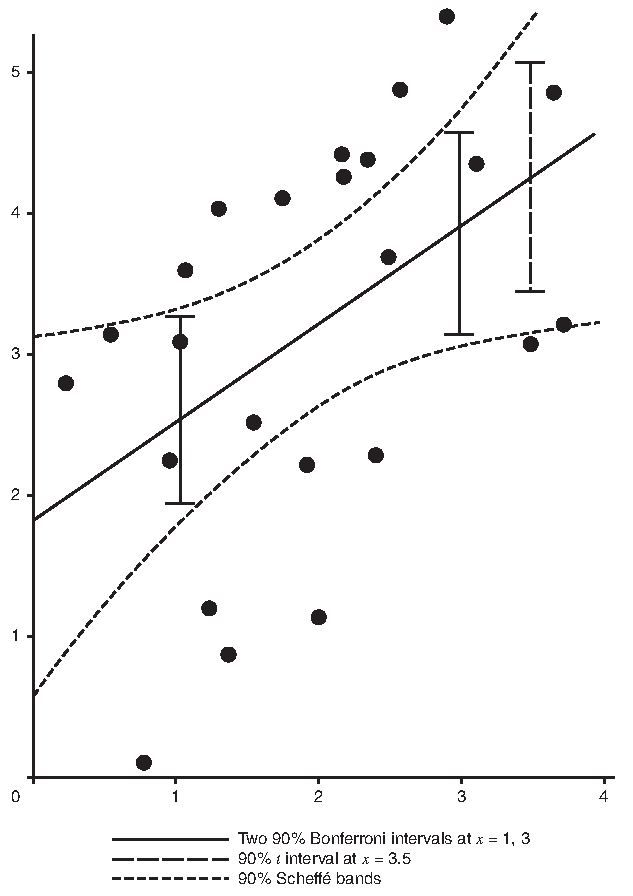
\includegraphics[width=.8\textwidth]{assets/chapter11/fig-11.3.3.pdf}
\caption{\autoref{tab:11.3.1}数据的Scheff\'e置信带、$t$区间（$x=3.5$处）及Bonferroni区间（$x=1$和$x=3$处）}\label{fig:11.3.3}
\end{figure}
最后指出，用Scheff\'e置信带等程序对观测$x$范围之外的$x$值作推断存在一个问题. 这些程序基于这样的假设：我们\emph{知道}总体回归函数对所有$x$都是线性的. 虽然假设回归函数在观测$x$的范围内线性可能合理，但向该范围之外的$x$作外推（extrapolation）通常不明智.\index{SI0891@外推}\semanticindexanchor{891:486} （观测范围之外没有数据，无法检查回归是否变成非线性.）这一提醒同样适用于\autoref{sec:11.3.5}的方法.
